\section{\glsentryshort{feba} Model in \glsentryshort{trace}}\label{sec:reflood_feba_trace}

The \gls{feba} facility was modeled using the TH system code \gls{trace}.
The model consists of a one-dimensional \textsc{VESSEL} component (to model the bundle test section),
a \textsc{PIPE} component (upper plenum of the test section), 
a \textsc{FILL} component (inlet flow and inlet temperature boundary conditions),
a \textsc{BREAK} component (outlet pressure boundary condition),
two \textsc{HTSTR} components (heater rods simulator and non-powered test section housing),
and a \textsc{POWER} components (imposed electrical boundary condition).

The \textsc{VESSEL} component was nodalized into $28$ hydraulic nodes of varying sizes between $60$ and $315 \ [mm]$.
Both \textsc{HTSTR} components were also nodalized into the sample number of coarse axial conduction nodes.
However, since a large axial temperature gradient is expected in a reflood transient,
the fine-mesh reflood flag in \gls{trace} was enabled.
As a result, each of the course conduction nodes is divided uniformly by $5$,
yielding a total of $142$ axial conduction nodes.
The main geometrical parameters and experimental conditions used to develop the \gls{trace} input model
are summarized in Table~\ref{tab:feba_trace},
and the nodalization of the model is illustrated in Fig.~\ref{fig:feba_nodalization}.

\begin{table}[ht]
    \myfloatalign
    \caption{Geometrical parameters and experimental conditions for the \Glsentryshort{feba} model in \Glsentryshort{trace}}
    \label{tab:feba_trace}
    \begin{tabularx}{\textwidth}{Xcc} \toprule
        \tableheadline{Parameter}		  & \tableheadline{Unit} & \tableheadline{Value} \\ \midrule
        Test section total length 		& $[m]$		& $4.114$ \\
        Total heated length 			    & $[m]$		& $3.9$ \\
        Flow area						          & $[m^2]$	& $3.901 \times 10^{-3}$\\
        Hydraulic diameter				    & $[mm]$	& $13.45$\\
        Rectangular housing width   	& $[mm]$	& $78.55$\\
        Rectangular housing thickness	& $[mm]$	& $6.5$\\
        Number of rods					      & $[-]$		& $25$\\
        Rod outer diameter				    & $[mm]$	& $10.75$\\
        Pitch-to-Diameter ratio			  & $[-]$		& $1.33$\\
        Number of spacer grids			  & $[-]$		& $7$\\
        Spacer grid flow obstruction	& $[\%]$	& $20$\\
        \multirow{3}{*}{Spacer grid axial locations}		& \multirow{3}{*}{$[m]$}		& $0.454, 0.999, 1.544,$\\
                                                        &                           & $2.089, 2.634, 3.179,$\\
                                                        &                           & $3.724$ \\
        \midrule
        Number of hydraulic nodes		  & $[-]$		& $28$ (varying length)\\
        \multirow{2}{*}{Number of axial nodes} 	& \multirow{2}{*}{$[-]$}		& $28$ (coarse)\\
                                		  &   		  & $142$ (fine)\\
        \midrule
        Inlet liquid temperature      & $[K]$		&  $312$ \\
        Inlet flow velocity				    & $[cm\cdot s^{-1}]$ & see Table~\ref{tab:feba_exp} \\
        System backpressure           & $[bar]$            & see Table~\ref{tab:feba_exp} \\
        \bottomrule
    \end{tabularx}
\end{table}

\begin{figure}[bth]
    \centering
    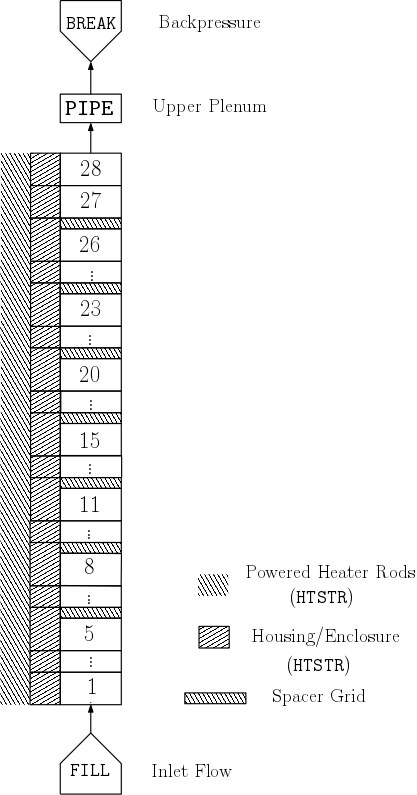
\includegraphics[width=0.65\textwidth]{../figures/febaNodalization/febaNodalization.png}
    \caption[\Glsentryshort{trace} nodalization of \glsentryshort{feba}]{Nodalization of FEBA experimental facility in \gls{trace}}
    \label{fig:feba_nodalization}
\end{figure}

\subsection{Base Case Simulation Results}

\subsection{Prior Uncertainty Propagation}
